\section{Question-1}

In this section we look at question 1. \\

Our script is given by:
\lstinputlisting{Question-1.py}

The printed results of the script are:

\lstinputlisting{Question-1.txt}

Our script produces the following plots.

The tests for our RNG produced for 1a):

\begin{figure}[h!]
  \centering
  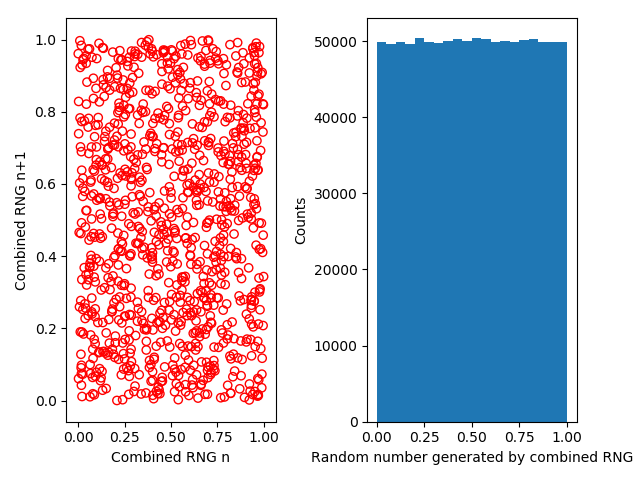
\includegraphics[width=0.9\linewidth]{./plots/RNG-test-results.png}
  \caption{Solution to Question 1a}
  \label{fig:fig1}
\end{figure}

For question 1b we used the following integral simplification:

\begin{alignat*}{3}
\int_{-\infty}^{\infty} \exp(-\alpha \cdot x^{2}) dx = 2 \cdot \int_{0}^{\infty} \exp(-\alpha \cdot x^{2}) dx = 2 \cdot [\int_{0}^{1} \exp(-\alpha \cdot x^{2}) dx + \int_{1}^{\infty} \exp(-\alpha \cdot x^{2}) dx] \\
= 2 \cdot [\int_{0}^{1} \exp(-\alpha \cdot x^{2}) dx + \int_{1}^{0} \exp(-\frac{\alpha}{y^{2}}) \cdot -\frac{dy}{y^{2}}] = 2 \cdot [\int_{0}^{1} \exp(-\alpha \cdot x^{2} + \frac{\exp(-\frac{\alpha}{x^{2}})}{x^{2}}) dx]
\end{alignat*}

Using the final integral form in combination with extended midpoint Romberg integration we got:
\begin{figure}[h!]
  \centering
  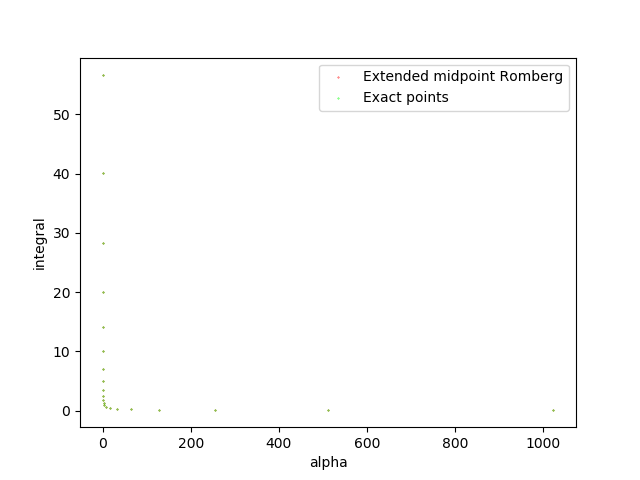
\includegraphics[width=0.9\linewidth]{./plots/gaussianintegral}
  \caption{Solution to Question 1b}
  \label{fig:fig2}
\end{figure}

\pagebreak
